%
% wrpc_hdl.tex
%
% White Rabbit PTP Core HDL.
%
\def\us{\char`\_}

\documentclass[a4paper, 12pt]{article}
%\documentclass{article}

\usepackage{fullpage}
\usepackage{pgf}
\usepackage{tikz}
\usetikzlibrary{arrows,automata,shapes}
\usepackage{multirow}
\usepackage{color}
\usepackage[latin1]{inputenc}
\usepackage{verbatim}
\usepackage{amsmath}
\usepackage{times,mathptmx}
\usepackage{chngcntr}
\usepackage{hyperref}
\usepackage[none]{hyphenat}
%\usepackage{draftwatermark}

%%%%%5% used in Tomeks %%%%%%%
\usepackage{listings}
\definecolor{light-gray}{gray}{0.95}
\usepackage{cancel}
%%%%%%%%%%%%%%%%%%%%%%%%%%%%%%%    fig/tomeksDrawings
%\usepackage{morefloats}

%\usepackage{amsfonts}
%\usepackage{amssymb}
%\usepackage{graphicx} 

%%%%%%%%%%%%%%%%%%%%%%%%%%%%%%%%%%%%%%%%%%%%%%%%%%%%%%%%%%%%%%%%%%%%%%%%%%%
% creating subsubsubsection notation
% src: http://www.latex-community.org/forum/viewtopic.php?f=5&t=791
%%%%%%%%%%%%%%%%%%%%%%%%%%%%%%%%%%%%%%%%%%%%%%%%%%%%%%%%%%%%%%%%%%%%%%%%%%%
\setcounter{secnumdepth}{6}
\renewcommand\theparagraph{\Alph{paragraph}}

\makeatletter
\renewcommand\paragraph{\@startsection{paragraph}{4}{\z@}%
                                     {-3.25ex\@plus -1ex \@minus -.2ex}%
                                     {0.0001pt \@plus .2ex}%
                                     {\normalfont\normalsize\bfseries}}
\renewcommand\subparagraph{\@startsection{subparagraph}{5}{\z@}%
                                     {-3.25ex\@plus -1ex \@minus -.2ex}%
                                     {0.0001pt \@plus .2ex}%
                                     {\normalfont\normalsize\bfseries}}
%\renewcommand{\thefootnote}{\fnsymbol{footnote}}
%\renewcommand{\thefootnote}{\alph{footnote}}

\counterwithin{paragraph}{subsubsection}
\counterwithin{subparagraph}{paragraph}
\makeatother
%%%%%%%%%%%%%%%%%%%%%%%%%%%%%%%%%%%%%%%%%%%%%%%%%%%%%%%%%%%%%%%%%%%%%%%%%%%%%%%%

\newcommand{\eqoffset}[1]{%
  {\ensuremath{%
      {\text{offset}}_{#1}}%
  }%
}
\newcommand{\eqdelay}[1]{{\text{delay}}_{#1}}
\newcommand{\eqasymm}{{\text{asymmetry}}}

\begin{document}

\title{White Rabbit PTP Core \\ HDL specification\\\normalsize
{version 1.0}\\\small{(01-03-2013)}}
\author{Grzegorz Daniluk\\ CERN BE-CO-HT}

\date{March 2013}
\maketitle
\thispagestyle{empty}

\begin{figure}[ht!]
  \centering
  \vspace{1.3cm}
  %\includegraphics[width=0.50\textwidth]{fig/wr_logo.png}
  \label{fig:wr_logo}
\end{figure}

\newpage

%\setcounter{page}{1}
%\begin{center}
%\large Revision History Table 
%\end{center} 
%
%\begin{table}[ht!]
%%\begin{table}[tbp]
%%\caption{White Rabbit Specification Revision History Table } 
%\centering
%\begin{tabular}{| c |  c | c | p{8cm}    |}          \hline
%\textbf{Version} & \textbf{Date} & \textbf{Authors} & \textbf{Description}  \\ 
% & &  &\\ \hline
%0.01 & 06/11/2012 & G.D.   & First draft for comments.  \\ \hline
%\end{tabular}
%\label{tab:revHist}
%\end{table}

\newpage

\newpage

\tableofcontents

\newpage

\section{Instantiating WRPC in your own HDL design}
\label{sec:wrpc_hdl}
This section describes the various options available to the users for instantiating and
parametrising the WRPC in their designs.

\begin{figure}[ht]
  \begin{center}
    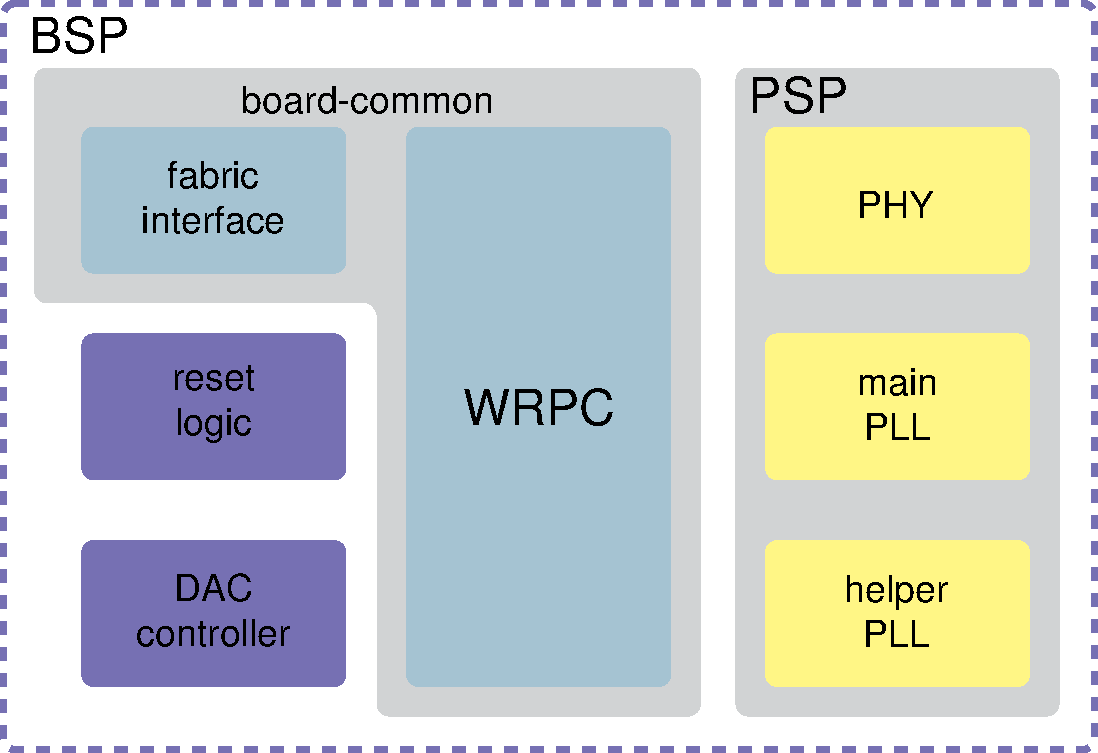
\includegraphics[width=.6\textwidth]{fig/wrpc_board.pdf}
    \caption{WRPC HDL abstraction hierarchy}
    \label{fig:wrpc_board}
  \end{center}
\end{figure}

The WRPC provides several levels of abstractions and VHDL modules, depending on the target
system. These are presented in Figure~\ref{fig:wrpc_board}. At the highest level of abstraction, the
WRPC provides Board Support Packages (BSPs), available for all officially supported boards. All BSP
modules share a common part (the ``board-common'' module) which encapsulates the WRPC core itself,
together with a selection of interfaces for connecting the core the the user FPGA
logic. Furthermore, each BSP also makes use of a Platform Support Package (PSP), which groups
together and instantiates all the FPGA-specific parts (typically hard IP provided by the FPGA
vendor), such as PHY, PLLs and clock buffers.

Thus, depending on the users' systems and needs, several scenarios might be available for
instantiating the WRPC into their designs.

\begin{description}
  \item[Option 1: Supported board.] In this simplest of scenarios, it will be enough to just
    instantiate the provided BSP into the users' designs and configure it via the provided generics.
  \item[Option 2: Supported FPGA platform.] The users could draw inspiration from an existing BSP
    based on the same platform, reusing the board-common module and PSP, while adapting the parts
    that are unique to their designs.
  \item[Option 3: Unsupported FPGA platform.] There is significant work involved in this
    scenario. In addition to providing the details for their board (just like for option 2), users
    also have to write their own PSP. It should be possible though to reuse the board-common
    module. Furthermore, if the unsupported platform is related to a supported one, it could be that
    the PHY and/or PLLs will also be reused, perhaps with minor adjustments.
\end{description}

When writing a new BSP or PSP, it's worth discussing it first in the
\href{http://www.ohwr.org/mailing_list/show?project_id=white-rabbit}{white-rabbit-dev} mailing
list. Perhaps there is already some preliminary support underway. It's also worth considering
sharing your work so that it can be merged with the project and added to the list of supported
platforms/boards.

The rest of this section describes the various modules in more detail. The WRPC module is presented
in Section~\ref{sec:hdl_wrpc}. The platform support modules are presented in
Section~\ref{sec:hdl_platform}, while the board support modules are presented in
Section~\ref{sec:hdl_board}.


\newpage
\section{Standard configuration}
\subsection{Generic parameters}
\label{sec:generics}

\begin{center}
  \begin{tabular}{|p{4cm}|p{2cm}|p{1.5cm}|p{6.5cm}|}
    \hline {\bf name} & {\bf type} & {\bf default value} & {\bf description} \\
    \hline
    \hline
    \texttt{g\_simulation} & integer & \texttt{0} & setting to '1' speeds up the simulation,
    must be set to '0' for synthesis\\
    \hline
    \texttt{g\_with\_external\_ \linebreak clock\_input} & boolean & \texttt{false} &
    enable external clock and 1-PPS inputs. The PLL inside WRPC will lock to
    external 10 MHz and 1-PPS signal when operating in GrandMaster mode\\
    \hline
  \end{tabular}
\end{center}

\subsection{Clocks and reset}
\label{basic:clk_rst}

\begin{figure}[ht]
  \begin{center}
    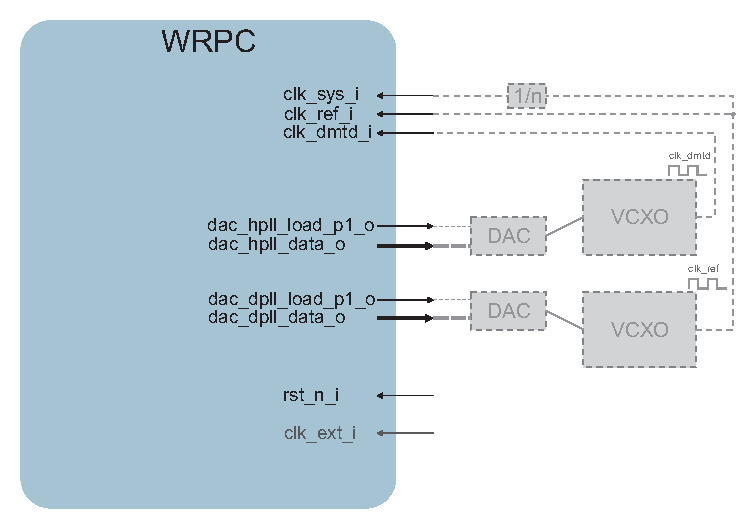
\includegraphics[width=.8\textwidth]{fig/basic_wrpc_clk.pdf}
    \caption{Mandatory clock signals and main reset of WRPC}
  \end{center}
\end{figure}


\begin{center}
  \begin{tabular}{|l|l|p{9cm}|}
    \hline
    %\multicolumn{3}{|l|}{\bf Signals description:}\\
    {\bf Signal name} & {\bf size} & {\bf description} \\
    \hline \hline
    \texttt{clk\_sys\_i} & 1 & main system clock, can be any frequency $\leq
    f_{clk\_ref\_i}$ e.g. 62.5 MHz\\
    \texttt{clk\_dmtd\_i} & 1 & DMTD offset clock (close to 62.5 MHz, e.g. 62.49 MHz)\\
    \texttt{clk\_ref\_i} & 1 & 125 MHz reference clock\\
    \hline
    \texttt{dac\_hpll\_load\_p1\_o} & 1 & validates DAC value on data port \\
    \texttt{dac\_hpll\_data\_o} & 16 & DAC value for tuning helper (DMTD) VCXO\\
    \texttt{dac\_dpll\_load\_p1\_o} & 1 & validates DAC value on data port \\
    \texttt{dac\_dpll\_data\_o} & 16 & DAC value for tuning main (ref) VCXO\\
    \hline
    \texttt{clk\_ext\_i} & 1 & [optional] external 10 MHz reference clock
    input for GrandMaster mode\\
    \texttt{rst\_n\_i} & 1 & main reset input, active-low (hold for at least 5
    \emph{clk\_sys} cycles)\\
    \hline
  \end{tabular}
\end{center}

\subsection{PHY interface}

\begin{figure}[ht]
  \begin{center}
    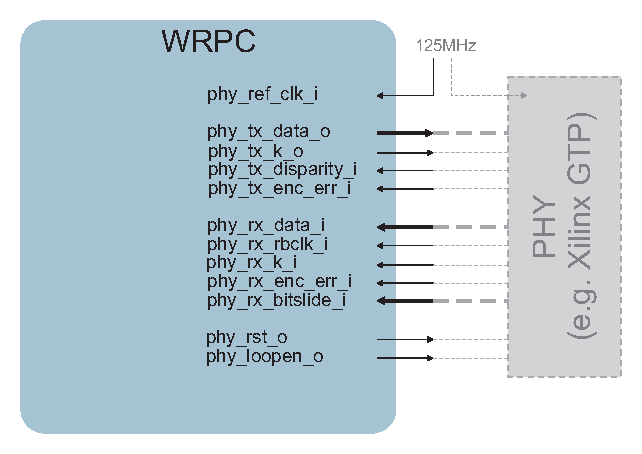
\includegraphics[width=.7\textwidth]{fig/wrpc_phyif.pdf}
    \caption{PHY interface of WRPC}
  \end{center}
\end{figure}

The interface connects WRPC with the Ethernet PHY layer IP-core. The interface is
generic, but currently two Gigabit Ethernet PHYs are tested and supported: Xilinx
8-bit GTP and 16-bit GTX SerDes. The signals' naming convention is the same as
in the GTP/GTX component definition.\\

{\bf Important !} If a WRPC user wants to use one of the supported PHYs (GTP,
GTX), they have to be taken from the White Rabbit HDL package instead of generating
them with the Xilinx Coregen tool. That is because WR developers have attached
additional logic to Xilinx GTP/GTX to improve its determinism.\\

\subsubsection{Fabric interface}
\label{sec:wrpc_fabric}

The Fabric interface is used for sending and receiving Ethernet frames. It consists 
of two pipelined Wishbone interfaces operating independently: 

\begin{itemize}
  \item \emph{WRF Source}: pipelined Wishbone Master, passes all the Ethernet frames
    received from a physical link to WRF Sink interface implemented in a
    user-defined module.
  \item \emph{WRF Sink}: pipelined Wishbone Slave, receives Ethernet frames from
    the WRF Source implemented in the user-defined module, and sends them to a
    physical link.
\end{itemize}

{\bf Address bus} can have one of the following values:

\begin{center}
\begin{tabular}{|c|l|}
  \hline {\bf decimal value} & {\bf meaning of data word on data bus}\\
  \hline
  \emph{0} & regular data (packet header and payload)\\
  \emph{1} & OOB (Out-of-band) data\\
  \emph{2} & status word\\
  \emph{3} & currently not used\\
  \hline
\end{tabular}
\end{center}

{\bf Status word} (sent when the value of address bus is \emph{2}) contains
various information about Ethernet frame's structure and type:
%\begin{figure}[ht]
  \begin{center}
    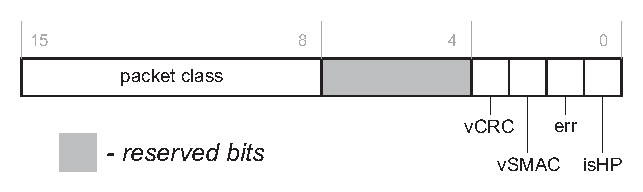
\includegraphics[width=.6\textwidth]{fig/status.pdf}
    %\caption{Status word format}
  \end{center}
%\end{figure}

\begin{itemize}
  \item[] \emph{isHP} - if \emph{1}, the frame is high priority
  \item[] \emph{err} - if \emph{1}, the frame contains an error
  \item[] \emph{vSMAC} - the frame contains a source MAC address (otherwise
    it will be assigned from WRPC configuration)
  \item[] \emph{vCRC} - the frame contains a valid CRC checksum
  \item[] \emph{packet class} - the packet class assigned by the classifier
    inside WRPC MAC module
\end{itemize}

OOB data is used for passing the timestamp-related information for the incoming and 
outgoing Ethernet frames. Each frame received from a physical link is
timestamped inside the WRPC and this value is passed as Rx OOB
data. On the other hand, for each transmitted frame the Tx timestamp can be read
from the Tx Timestamping Interface (section \ref{sec:txts}) together with a unique
frame number assigned in Tx OOB. Therefore, the format of OOB differs between Rx
and Tx frames.\\

{\bf Tx OOB format}:

%\begin{figure}[ht]
  \begin{center}
    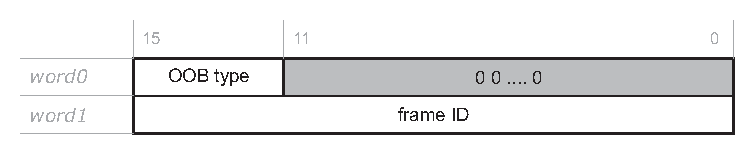
\includegraphics[width=.7\textwidth]{fig/oob_tx.pdf}
    %\caption{Tx OOB data format}
    %\label{fig:fabric_adv:tx_oob}
  \end{center}
%\end{figure}

\begin{itemize}
  \item[] \emph{OOB type}: "0001" means Tx OOB
  \item[] \emph{frame ID}: ID of the frame being sent. It is later output
    through the \emph{Tx Timestamping interface} to associate Tx timestamp with
    appropriate frame. Frame ID = 0 is reserved for PTP packets inside WRPC
    and cannot be used by user-defined modules.
\end{itemize}

{\bf Rx OOB format}:
%\begin{figure}[ht]
  \begin{center}
    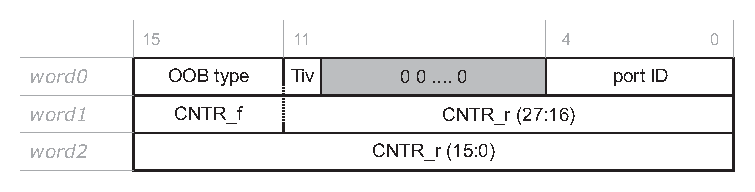
\includegraphics[width=.7\textwidth]{fig/oob_rx.pdf}
    %\caption{Rx OOB data format}
    %\label{fig:fabric_adv:rx_oob}
  \end{center}
%\end{figure}

\begin{itemize}
  \item[] \emph{OOB type}: "0000" means Rx OOB
  \item[] \emph{Tiv}: timestamp invalid. When this bit is set to '1', the PPS
    generator inside WRPC is being adjusted which means the Rx timestamp is not
    reliable.
  \item[] \emph{port ID}: the ID of a physical port on which the packet was
    received. In case of WRPC, this field is always 0, because there is only one
    physical port available.
  \item[] \emph{CNTR\_f}: least significant bits of the Rx timestamp generated on
    the falling edge of the reference clock.
  \item[] \emph{CNTR\_r}: Rx timestamp generated on the rising edge of the reference
    clock.
\end{itemize}

\begin{figure}
  \begin{center}
    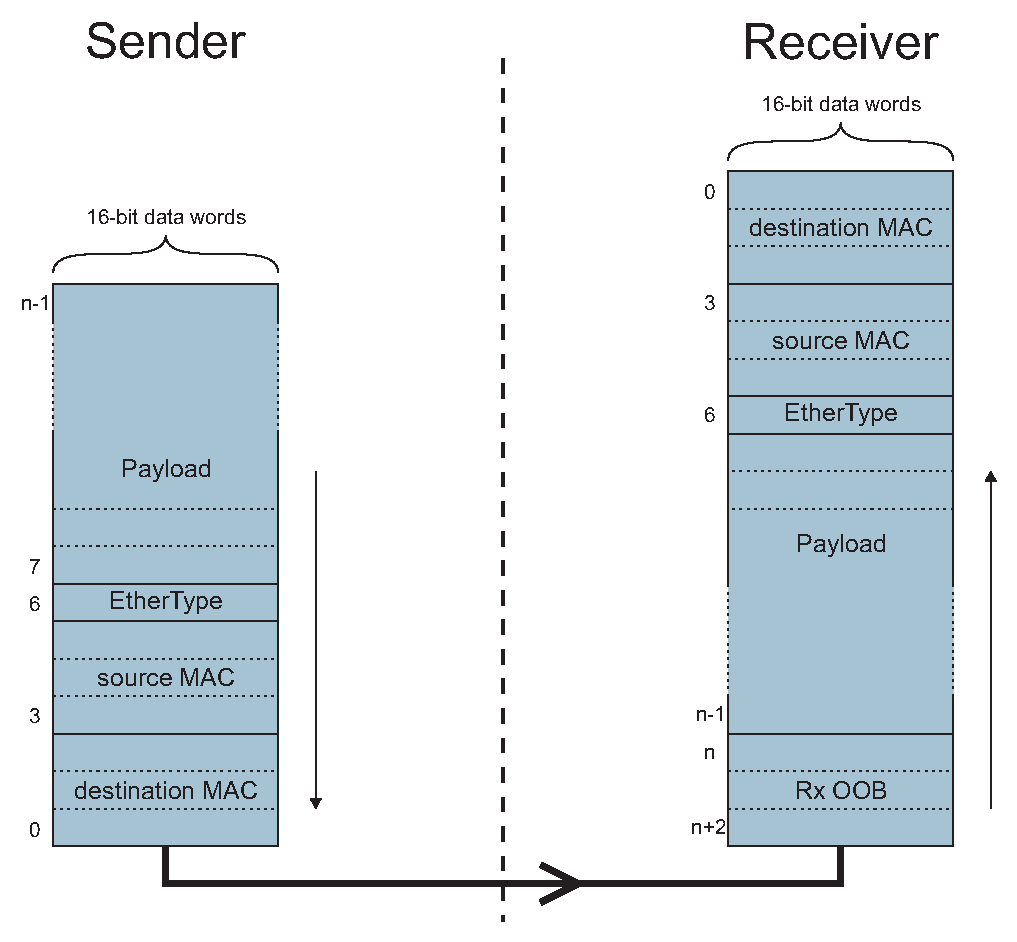
\includegraphics[width=.6\textwidth]{fig/basic_wrf_data.pdf}
    \caption{Data words that make the Ethernet frame}
    \label{fig:fabric:simple_data}
  \end{center}
\end{figure}

Figure \ref{fig:fabric:simple_data} presents data words fed to the WRF
data bus by the sender and the information got at the receiving side. Please
note that the CRC checksum is calculated and inserted automatically inside the
WRPC and user-defined module doesn't care about it. The Ethernet frame received
from the WR Fabric interface may contain additional OOB data suffixed. It has to
be received (acknowledged) by the user-defined module, but can be simply discarded.

\newparagraph{Examples}
Figure \ref{fig:fabric:simple_tx} shows a very simple WR Fabric cycle. The WRF
Source of user-defined module sends there an Ethernet frame containing even
number of bytes.

\begin{figure}
  \begin{center}
    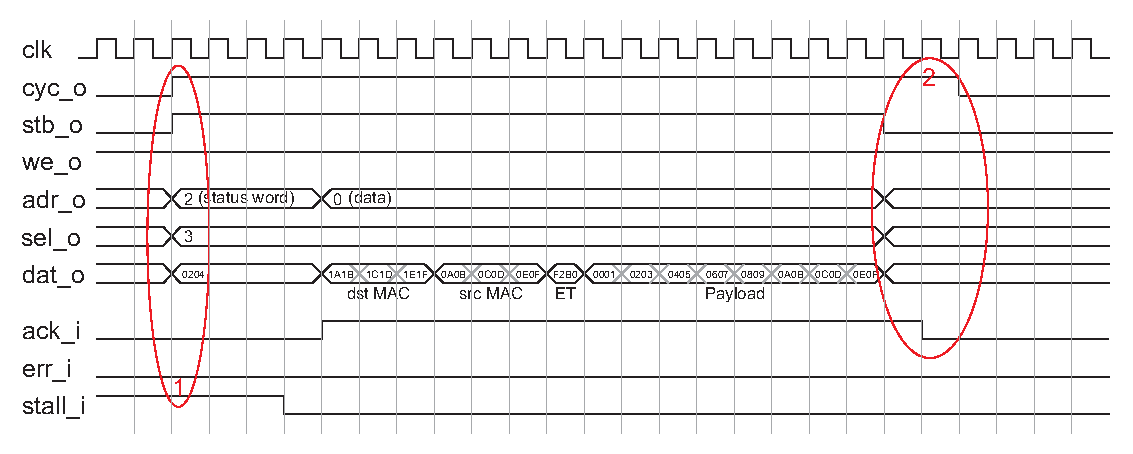
\includegraphics[width=\textwidth]{fig/basic_wrf_cycle_simple.pdf}
    \caption{Simple WR Fabric cycle - user-defined module sending packet}
    \label{fig:fabric:simple_tx}
  \end{center}
\end{figure}

\begin{enumerate}
  \item The WRF Source in user-defined module starts the cycle by asserting
    \emph{cyc\_o}, \emph{stb\_o} and putting a status word to the data bus.
    However, since WRF Sink set \emph{stall} signal to active state, Source has
    to wait until Sink is ready to receive data.
  \item After the last word is transmitted, the WRF Source sets \emph{stb\_o} back
    to \emph{0}, but waits until Sink acknowledges all the words transmitted in
    the cycle (\emph{ack\_i} line). The cycle ends when \emph{cyc\_o} goes back
    to the low state.
\end{enumerate}

Figure \ref{fig:fabric:sel} shows again a very simple WR Fabric cycle where
user-defined WRF Source sends an Ethernet frame to the WRPC. This time though,
the frame contains odd number of bytes, therefore the \emph{sel} line is used to
signal this fact to WRF Sink inside the WRPC (1).

\begin{figure}
  \begin{center}
    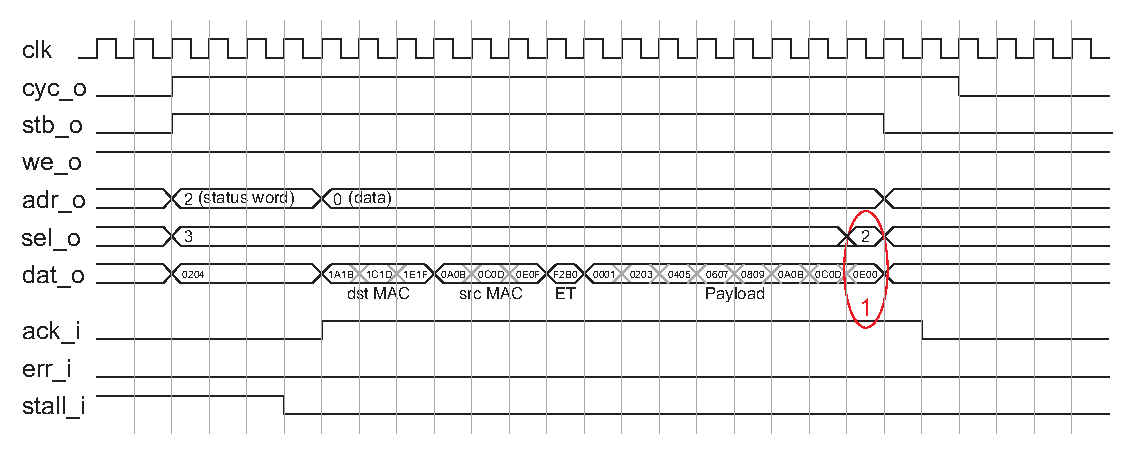
\includegraphics[width=\textwidth]{fig/basic_wrf_cycle_sel.pdf}
    \caption{Simple WR Fabric cycle - user-defined module sending packet(odd
    number of bytes in the payload)}
    \label{fig:fabric:sel}
  \end{center}
\end{figure}

Figure \ref{fig:fabric:cyc} presents more complicated Fabric cycle where an
Ethernet frame is received from WRF Source in the WRPC (output signals in the
diagram are driven by WRF Source on the WRPC side): 

\begin{figure}
  \begin{center}
    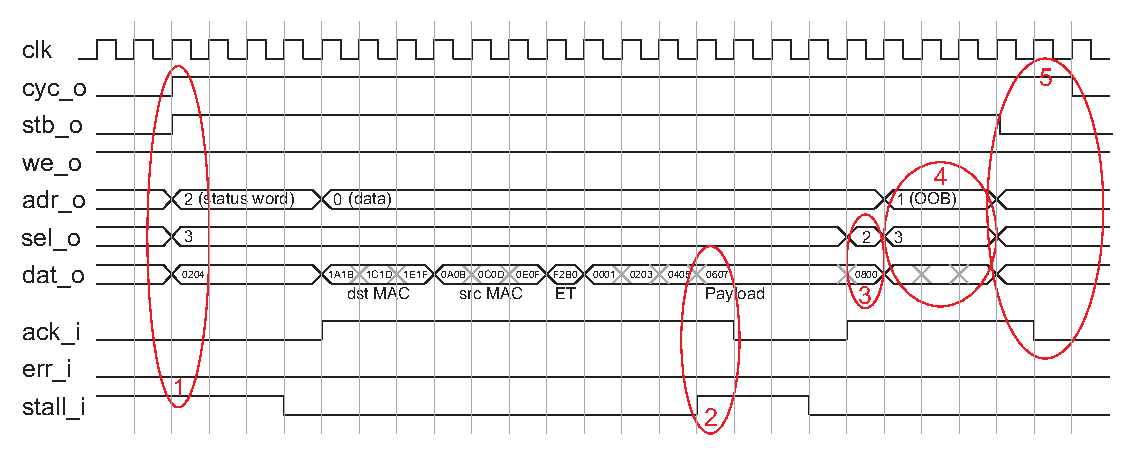
\includegraphics[width=\textwidth]{fig/basic_wrf_cycle.pdf}
    \caption{WR Fabric cycle}
    \label{fig:fabric:cyc}
  \end{center}
\end{figure}
\begin{enumerate}
  \item The WRF Source starts the cycle by asserting \emph{cyc\_o}, \emph{stb\_o}
    and putting a status word to the data bus. However, since WRF Sink set 
    \emph{stall} signal to active state, Source has to wait until Sink is ready
    to receive data.
  \item While the payload of the Ethernet frame is being transmitted, Sink
    stalls the cycle. The WRF Source pauses the transmission until Sink becomes
    ready to process the rest of the data. During that time \emph{stb\_o} has to
    remain in a high state.
  \item The Ethernet frame contains an odd number of bytes, so only half of last
    word of payload carries a valid data. \emph{Sel\_o} is used to signal this
    fact to WRF Sink.
  \item After the whole payload is transmitted, Source may additionally sent Rx
    OOB data. It contains some internal WRPC data that should be acknowledged
    by Sink, but discarded in the user's module.
  \item After the last word is transmitted, the WRF Source sets \emph{stb\_o} back
    to \emph{0}, but waits until Sink acknowledges all the words transmitted in
    the cycle (\emph{ack\_i} line). The cycle ends when \emph{cyc\_o} goes back
    to the low state.
\end{enumerate}

WRF Sink can use the \emph{stall} line to pause the frame transmission if it cannot
process the flow of data coming from WRF Source. However, if some more serious
problem appears on the receiving side, the \emph{err} line can be used to
immediately break the cycle. This situation is presented in figure
\ref{fig:fabric:cycerr}:

\begin{figure}
  \begin{center}
    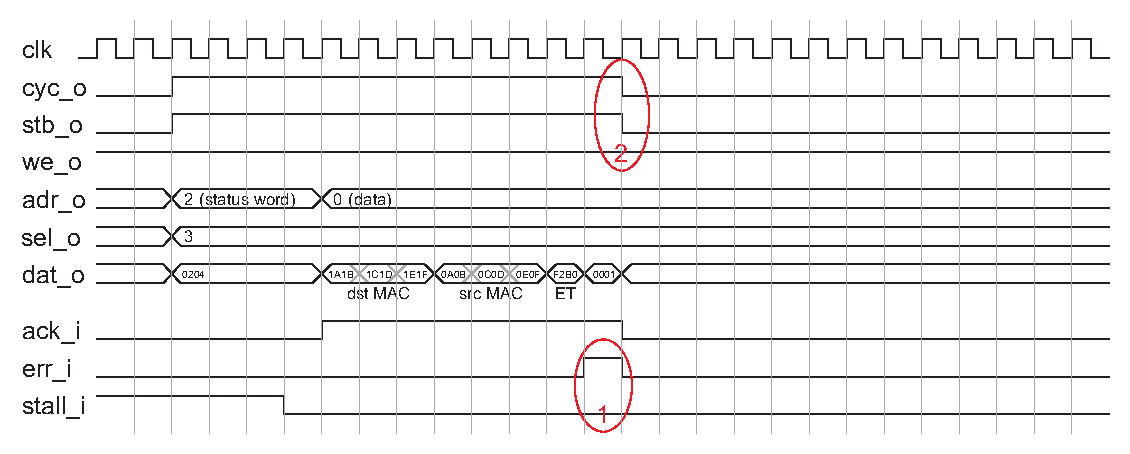
\includegraphics[width=\textwidth]{fig/basic_wrf_cycle_err.pdf}
    \caption{WR Fabric cycle interrupted with an error line}
    \label{fig:fabric:cycerr}
  \end{center}
\end{figure}

\begin{enumerate}
  \item WRF Sink wants to break a bus cycle, so it drives \emph{err\_i} high.
  \item WRF Source breaks the cycle immediately after receiving an error indicator
    from the WRF Sink.
\end{enumerate}

\newparagraph{SystemVerilog model}
The SystemVerilog simulation model of the WR Fabric interface (both WRF Source and 
WRF Sink) can be found in the \emph{wr-cores} git repository
(git://ohwr.org/hdl-core-lib/wr-cores.git) and consists of the files:
\begin{itemize}
  \item \emph{sim/if\_wb\_master.svh}
  \item \emph{sim/if\_wb\_slave.svh}
  \item \emph{sim/wb\_packet\_source.svh}
  \item \emph{sim/wb\_packet\_sink.svh}
\end{itemize}

The testbench example using the simulation model of WR Fabric interface can
be found in the zip archive attached to this documentation.


\subsubsection{Timecode interface}
\label{sec:wrpc_timecode}

%\begin{figure}[ht]
%  \begin{center}
%    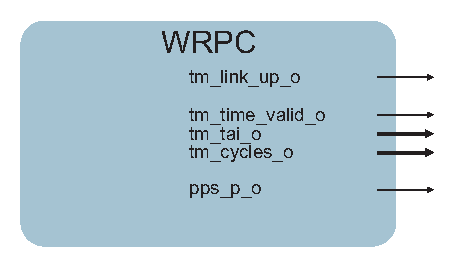
\includegraphics[width=.5\textwidth]{fig/basic_wrpc_tm.pdf}
%    \caption{Timecode output interface of WRPC}
%  \end{center}
%\end{figure}

Timecode interface provides current time to the other HDL modules in a form that
can be easily used. It consists of: a 1-PPS and a UTC timecode
aligned to the time of WR Master.


\subsection{GPIO/UART/I2C/1-Wire/SPI interfaces}
\label{sec:wrpc_periph}

%\begin{figure}[ht]
%  \begin{center}
%    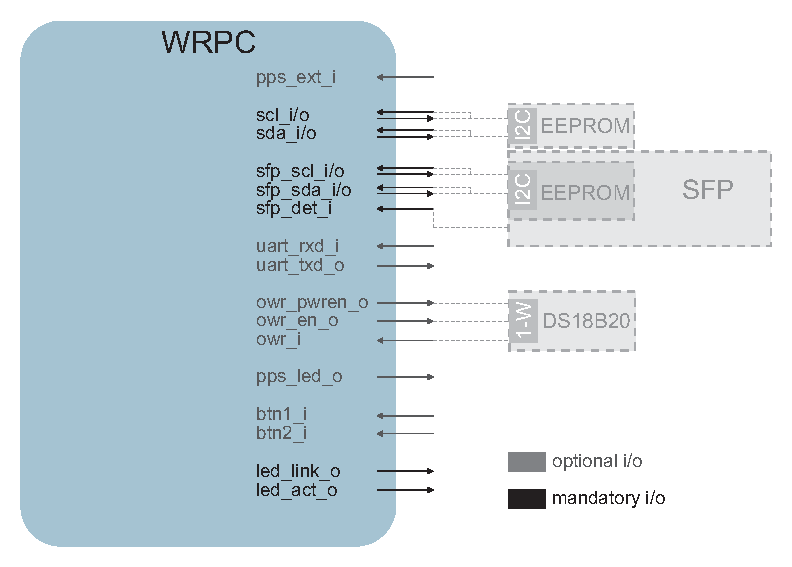
\includegraphics[width=.9\textwidth]{fig/basic_wrpc_gpio.pdf}
%    \caption{Other interfaces of WRPC}
%  \end{center}
%\end{figure}

Several hardware peripherals can be connected to the White Rabbit PTP Core. It
has:
\begin{itemize}
  \item UART - provides access to the WR PTP Core user shell
  \item 1-Wire - access to a digital thermometer for an on-board temperature and
    unique ID (used to generate a default MAC address of the WR port)
  \item SFP $I^2C$ - access to the SFP EEPROM, to read its ID and math with the
    calibration values
  \item SPI - access to the Flash memory, used to store calibration
    parameters and init script
  \item EEPROM $I^2C$ - [optional] access to the EEPROM memory, used to store
    calibration parameters and init script - currently SPI Flash is the
    preferred storage, however, EEPROM can still be used if needed.
\end{itemize}


\newpage
\appendix
\section{Appendix: Advanced options}
{\color{red} {\bf Information presented in this part should be used only
    by users with expert knowledge of the White Rabbit Protocol and on their own
responsibility}}
\subsection{Generic parameters}
\label{sec:adv:generics}

\begin{center}
  \begin{tabular}{|p{3.7cm}|p{3.3cm}|p{2.2cm}|p{5cm}|}
    \hline {\bf name} & {\bf type} & {\bf default value} & {\bf description} \\
    \hline
    \hline
    \texttt{g\_phys\_uart} & boolean & \texttt{true} & enable physical UART interface\\
    \hline
    \texttt{g\_virtual\_uart} & boolean & \texttt{false} & enable virtual UART interface\\
    \hline
    \texttt{g\_aux\_clks} & integer & \texttt{1} & number of aux clocks syntonized by WRPC to WR
    timebase\\
    \hline
    \texttt{g\_rx\_buffer\_size} & integer & \texttt{1024} & size of Rx buffer in WRPC MAC module,
    default value is 1024 and should not be changed\\
    \hline
    \texttt{g\_dpram\_initf} & string & \texttt{""} & filename of compiled WRPC software, to be
    stored in WRPC memory during the synthesis (default is \emph{wrc.ram}
    created by compiling WRPC software from \emph{wrpc-sw} git repository)\\
    \hline
    \texttt{g\_dpram\_initv} & t\_xwb\_dpram\_init &
    \texttt{c\_xwb\_ \linebreak dpram\_init \linebreak \_nothing} & VHDL array to initialize WRPC
    internal memory\\
    \hline
    \texttt{g\_dpram\_size} & integer & \texttt{22528} & size of RAM used by WRPC software (in 32-bit
    words), default value is 22528 and should not be changed\\
    \hline
    \texttt{g\_interface\_ \linebreak mode} & t\_wishbone\_ \linebreak interface\_mode &
    \texttt{PIPELINED} & external Wishbone Slave interface mode
    [PIPELINED/CLASSIC]\\
    \hline
    \texttt{g\_address\_ \linebreak granularity} & t\_wishbone\_ \linebreak
    address\_granularity & \texttt{WORD} & granularity of address bus in
    external Wishbone Slave interface [BYTE/WORD]\\
    \hline
    \texttt{g\_aux\_sdb} & t\_sdb\_device & \texttt{c\_wrc\_ \linebreak
    periph3\_ \linebreak sdb} & structure providing SDB Wishbone description of
    WRPC, when connected to SDB Wishbone Crossbar, this parameter is optional
    and can be unassigned\\
    \hline
  \end{tabular}
\end{center}

\subsection{Aux clocks}

\begin{figure}[ht]
  \begin{center}
    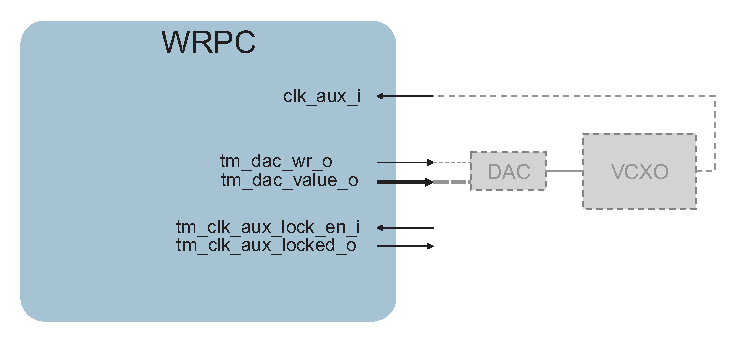
\includegraphics[width=.8\textwidth]{fig/adv_wrpc_clk.pdf}
    \caption{Aux clock synchronization interface}
  \end{center}
\end{figure}

The WRPC can syntonize auxiliary clock signals to the White Rabbit timebase. It
is done with a similar PLL that is used to discipline the local reference clock
(section \ref{basic:clk_rst}). WRPC provides tuning values for the VCXO producing
clock signal which is connected to \emph{clk\_aux\_i}.

\begin{center}
  \begin{tabular}{|l|l|p{9cm}|}
    \hline
    \multicolumn{3}{|l|}{\bf Signals description:}\\
    {\bf name} & {\bf size} & {\bf description} \\
    \hline \hline
    \texttt{clk\_aux\_i} & g\_aux\_clks & [optional] vector of auxiliary
    clocks that will be disciplined to WR timebase\\
    \hline
    \texttt{tm\_dac\_value\_o} & 24 & DAC value for tuning auxiliary clock
    (\emph{clk\_aux\_i})\\
    \texttt{tm\_dac\_wr\_o} & 1 & validates auxiliary DAC value\\
    \texttt{tm\_clk\_aux\_lock\_en\_i} & 1 & enable locking auxiliary clock to
    internal WR clock\\
    \texttt{tm\_clk\_aux\_locked\_o} & 1 & auxiliary clock locked to internal WR
    clock\\
    \hline
  \end{tabular}
\end{center}

\subsection{Fabric interface}

Address bus can have one of the following values:
\begin{center}
\begin{tabular}{|c|l|}
  \hline {\bf decimal value} & {\bf meaning of data word on data bus}\\
  \hline
  \emph{0} & regular data (packet header and payload)\\
  \emph{1} & OOB (Out-of-band) data\\
  \emph{2} & status word\\
  \emph{3} & currently not used\\
  \hline
\end{tabular}
\end{center}

{\bf Status word} (sent when the value of address bus is \emph{2}) contains
various information about Ethernet frame's structure and type:
\begin{figure}[ht]
  \begin{center}
    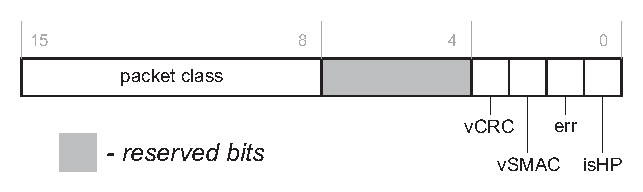
\includegraphics[width=.6\textwidth]{fig/status.pdf}
    \caption{Status word format}
  \end{center}
\end{figure}

\begin{itemize}
  \item[] \emph{isHP} - if \emph{1}, the frame is high priority
  \item[] \emph{err} - if \emph{1}, the frame contains an error
  \item[] \emph{vSMAC} - the frame contains a source MAC address (otherwise
    it will be assigned from WRPC configuration)
  \item[] \emph{vCRC} - the frame contains a valid CRC checksum
  \item[] \emph{packet class} - the packet class assigned by the classifier
    inside WRPC MAC module
\end{itemize}

OOB data is used for passing the timestamp-related information for the incoming and 
outgoing Ethernet frames. Each frame received from a physical link is
timestamped inside the WRPC and this value is passed as Rx OOB
data. On the other hand, for each transmitted frame the Tx timestamp can be read
from the Tx Timestamping Interface (section \ref{sec:txts}) together with a unique
frame number assigned in Tx OOB. Therefore, the format of OOB differs between Rx
and Tx frames.\\

{\bf Tx OOB format} (figure \ref{fig:fabric_adv:tx_oob}):

\begin{figure}[ht]
  \begin{center}
    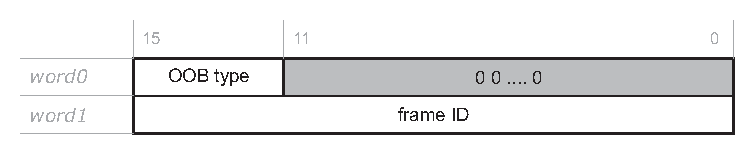
\includegraphics[width=.7\textwidth]{fig/oob_tx.pdf}
    \caption{Tx OOB data format}
    \label{fig:fabric_adv:tx_oob}
  \end{center}
\end{figure}

\begin{itemize}
  \item[] \emph{OOB type}: "0001" means Tx OOB
  \item[] \emph{frame ID}: ID of the frame being sent. It is later output
    through the \emph{Tx Timestamping interface} to associate Tx timestamp with
    appropriate frame. Frame ID = 0 is reserved for PTP packets inside WRPC
    and cannot be used by user-defined modules.
\end{itemize}

{\bf Rx OOB format} (figure \ref{fig:fabric_adv:rx_oob}):
\begin{figure}[ht]
  \begin{center}
    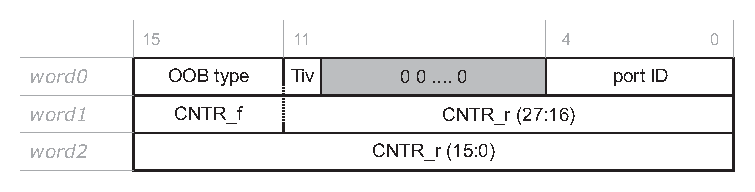
\includegraphics[width=.7\textwidth]{fig/oob_rx.pdf}
    \caption{Rx OOB data format}
    \label{fig:fabric_adv:rx_oob}
  \end{center}
\end{figure}

\begin{itemize}
  \item[] \emph{OOB type}: "0000" means Rx OOB
  \item[] \emph{Tiv}: timestamp invalid. When this bit is set to '1', the PPS
    generator inside WRPC is being adjusted which means the Rx timestamp is not
    reliable.
  \item[] \emph{port ID}: the ID of a physical port on which the packet was
    received. In case of WRPC, this field is always 0, because there is only one
    physical port available.
  \item[] \emph{CNTR\_f}: least significant bits of the Rx timestamp generated on
    the falling edge of the reference clock.
  \item[] \emph{CNTR\_r}: Rx timestamp generated on the rising edge of the reference
    clock.
\end{itemize}

\subsection{External Wishbone Slave/Master interface}

\begin{figure}[ht]
  \begin{center}
    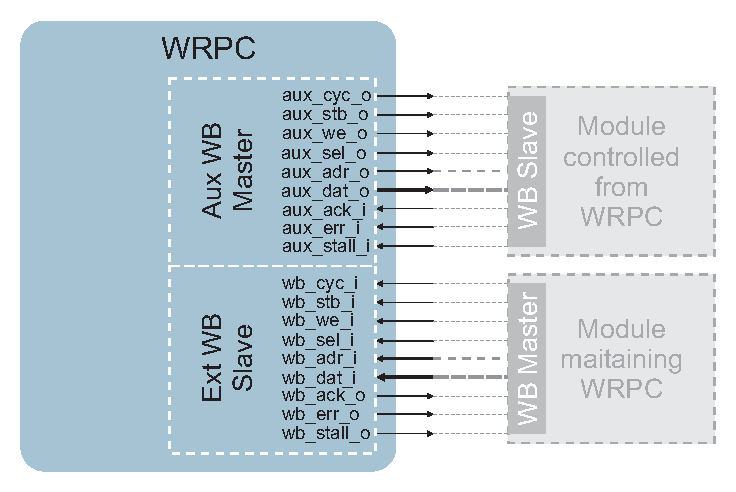
\includegraphics[width=.7\textwidth]{fig/wrpc_wb.pdf}
    \caption{External Wishbone interfaces of WRPC}
  \end{center}
\end{figure}

{\bf Aux WB Master} is a Pipelined Wishbone Master interface. It is connected
through the Wishbone Crossbar inside the White Rabbit PTP Core to the LM32 soft-core
processor (instantiated inside the WRPC). It can optionally be used to control
any user-defined module having a Pipelined Wishbone Slave interface. In that case, the WRPC software
has to be modified to control additional modules connected to the \emph{Aux WB
Master} interface.\\

{\bf Ext WB Slave} is a Wishbone Slave interface that operates in Pipelined or
Classic mode (selected with \emph{g\_interface\_mode} generic), with the address bus
granularity set with \linebreak \emph{g\_address\_granularity} generic. It gives the access
to control all the WRPC internals. In the WRPC reference design it is connected to
the Gennum GN4124 IP-core and used to upload WRPC software to its internal memory.\\

HDL modules accessible through \emph{Ext WB Slave} interface:
\begin{center}
  \begin{tabular}{|l|l|}
    \hline {\bf module name} & {\bf offset (bytes)}\\
    \hline
    WRPC internal memory & 0x00000\\
                Mini NIC & 0x20000\\
                Endpoint & 0x20100\\
                Soft PLL & 0x20200\\
           PPS generator & 0x20300\\
                  Syscon & 0x20400\\
                    UART & 0x20500\\
           1-Wire Master & 0x20600\\
           Aux WB Master & 0x20700\\
    \hline
  \end{tabular}
\end{center}

\subsubsection{Tx Timestamping interface}
\label{sec:txts}

The Tx Timestamping interface provides the timestamps generated inside WRPC for each
Ethernet frame transmitted from user-defined module through the WRF Sink interface.\\



\newpage
\bibliographystyle{unsrt}
\bibliography{references}

%\newpage
%\appendix
\section{Appendices}

\subsection{Simple top design with WRPC}
\label{app:top_design}

\begin{center}
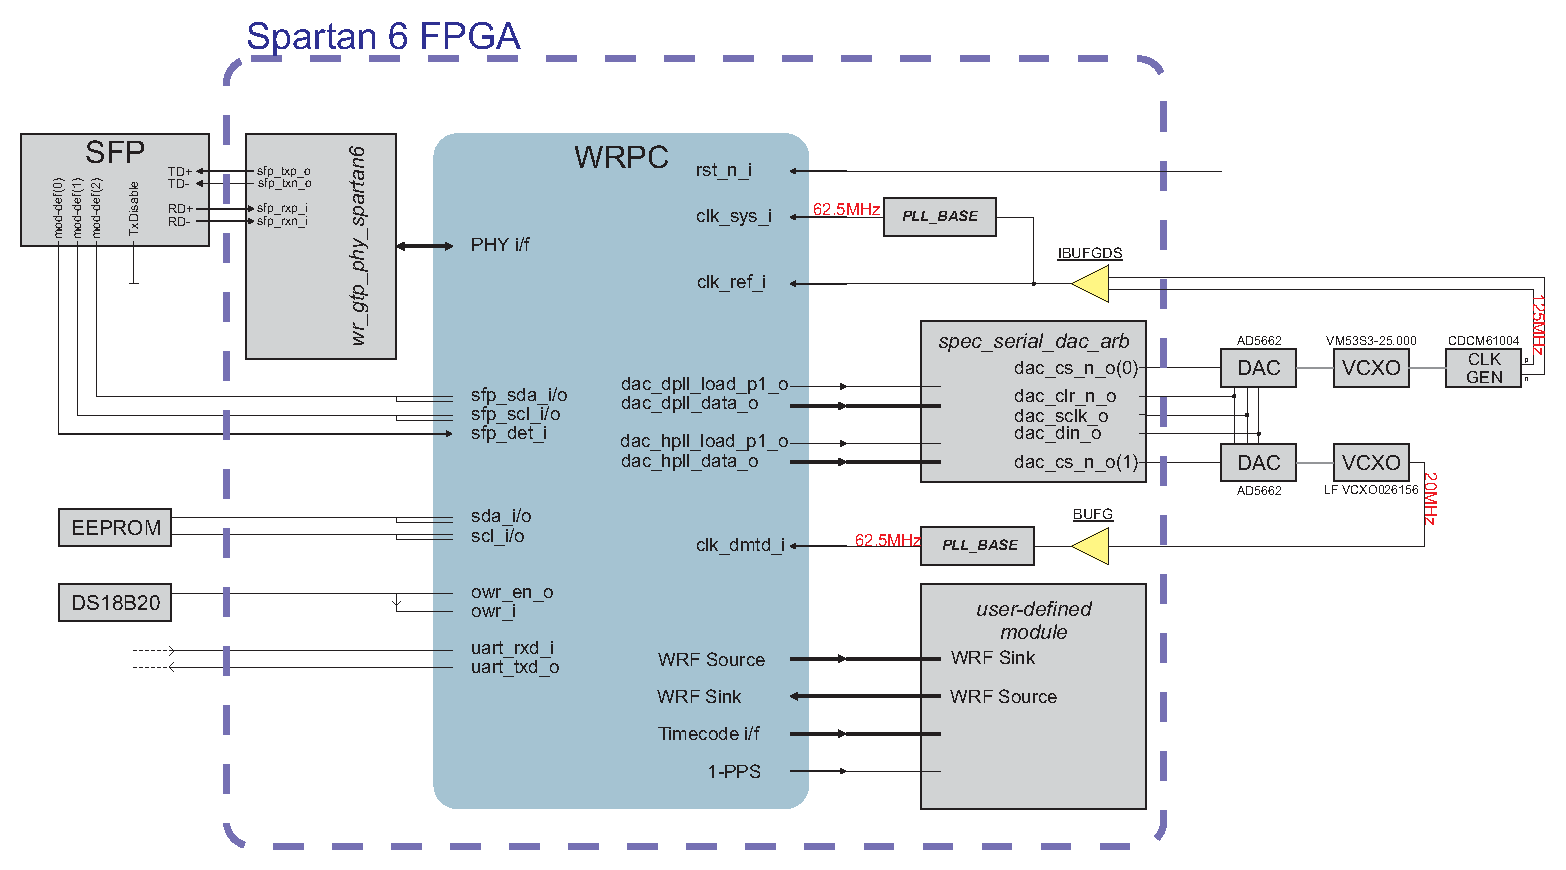
\includegraphics[width=.9\textheight, angle=90]{fig/basic_top.pdf}
\end{center}

%\newpage
%\subsection{WR Fabric testbench example}
%\label{app:fabric_tb}
%
%\begin{lstlisting}
%/* A small testbench demonstrating how to send Ethernet packets 
% * over WRPC's Fabric interface.*/
%
%`include "if_wb_master.svh"
%`include "if_wb_slave.svh"
%`include "wb_packet_sink.svh"
%`include "wb_packet_source.svh"
%
%`timescale 1ns/1ns
%
%module main;
%
%   reg                   clk = 0;
%   reg                   rst = 0;
%
%   /* Clock / reset generation */
%   initial #100 rst = 1;
%   always #10 clk <= ~clk;
%
%   /* Packet Sink Wishbone interface (slave) - inputs packets,
%    * simulating a MAC TX input.*/
%   IWishboneSlave
%     #(
%       .g_data_width(16),
%       .g_addr_width(2))
%   U_WB_Slave
%     (
%      .clk_i(clk),
%      .rst_n_i(rst)
%      );
%
%   /* Packet Sink Wishbone interface (slave) - inputs packets,
%    * simulating a MAC TX input.*/
%   IWishboneMaster
%     #(
%       .g_data_width(16),
%       .g_addr_width(2))
%   U_WB_Master
%     (
%      .clk_i(clk),
%      .rst_n_i(rst)
%      );
%
%   assign U_WB_Slave.adr = U_WB_Master.adr;
%   assign U_WB_Slave.dat_i = U_WB_Master.dat_o;
%   assign U_WB_Slave.cyc = U_WB_Master.cyc;
%   assign U_WB_Slave.stb = U_WB_Master.stb;
%   assign U_WB_Slave.sel = U_WB_Master.sel;
%   assign U_WB_Slave.we = U_WB_Master.we;
%
%   assign U_WB_Master.ack = U_WB_Slave.ack;
%   assign U_WB_Master.stall = U_WB_Slave.stall;
%   assign U_WB_Master.rty = U_WB_Slave.rty;
%   assign U_WB_Master.err = U_WB_Slave.err;
%
%   /* Packet Transmission process */
%   initial begin
%
%      /* Create a Packet Source object: WBPacketSource class
%       * takes Ethernet packets and converts them to 
%       * Wishbone transactions .*/
%      WBPacketSource src = new(U_WB_Master.get_accessor());
%      EthPacket pkt, template = new;
%      EthPacketGenerator gen = new;
%
%      int i;
%
%      /* Force the WB Master to make some mess on the bus by 
%       * throttling transfer rate (random empty slots).*/
%      U_WB_Master.settings.gen_random_throttling = 1;
%      U_WB_Master.settings.throttle_prob = 0.05;
%
%      /* Size range: 64 to 128 bytes */
%      gen.set_size(64, 128);
%
%      /* Payload = sequence of increasing bytes */
%      gen.set_randomization(EthPacketGenerator::SEQ_PAYLOAD);
%
%      template.src = '{ 'hca, 'hfe, 'hba, 'hbe, 'h00, 'h01 };
%      template.dst = '{ 'hff, 'hff, 'hff, 'hff, 'hff, 'hff };
%      template.ethertype = 'h1234;
%
%      /* Set template header for all generated packets 
%       * (i.e. MAC, Ethertype). */
%      gen.set_template(template);
%
%      /* Wait until reset goes low */
%      #200;
%
%      for (i = 0; i < 10; i++) begin
%         pkt = gen.gen();
%         $display("Send %d\n", i);
%         src.send(pkt);
%      end
%   end
%
%   initial begin
%      /* Create a Packet Sink object: WBPacketSink class
%       * decodes Wishbone transactions into Ethernet packets.*/
%      WBPacketSink snk = new (U_WB_Slave.get_accessor());
%      EthPacket pkt;
%
%      int i;
%
%      /* Make the WB Slave sometimes stall the Wishbone link,
%       * to demonstrate various conditions on the bus.*/
%      U_WB_Slave.settings.gen_random_stalls = 1;
%      U_WB_Slave.settings.stall_prob = 0.05;
%      U_WB_Slave.settings.stall_min_duration = 1;
%      U_WB_Slave.settings.stall_max_duration = 5;
%
%      /* Wait until reset goes low */
%      #200;
%
%      /* Print all received packets */
%      forever begin
%         snk.recv(pkt);
%         pkt.dump();
%      end
%   end
%
%endmodule // main
%\end{lstlisting}


\end{document}
